\section{Versuchsziel}
\label{sec:Versuchsziel}
Das Ziel des Experiments ist es, die Wellenlänge eines Lasers und die Brechungsindizes zweier Gase mit Hilfe eines Michelson-Interferometers zu bestimmen.

\section{Theorie}
\label{sec:Theorie}

In letzter Zeit ist es Wissenschaftlern gelungen, Gravitationswellen nachzuweisen.
Hierzu wurde ein Michelson-Interferometer benutzt, da es dazu geeignet ist, Wellenlängen, sowie deren absolute Änderung zu messen.
Zusätzlich können auch Brechungsindizes gemessen werden.
Das Michelson-Interferometer selbst stützt sich auf das Interferenzprinzip, auf welches im Folgenden weiter eingegangen wird.\\
\subsection{Interferenz des Lichtes}
Im Allgemeinen kann Licht als elektromagnetische Welle der Form
\begin{equation}
  \vec{E}(x,t) = \vec{E_0}\exp{(i(\vec{k}\vec{x}-\omega t -\delta))}, \label{eqn:1}
\end{equation}
mit Ort $\vec{x}$ und Zeit $t$, sowie Wellenvektor $\vec{k}$, Frequenz $\omega$ und Phasenkonstante $\delta$, angenommen werden, wobei sie sich nur in ihrer Intensität
\begin{equation}
  I \propto |\vec{E}|²
\end{equation}
messbar macht.
Da diese elektromagnetischen Wellen den Maxwell-Gleichungen unterliegen, gilt die lineare Superposition, wodurch sich zwei Wellen einfach addieren lassen.
Aus Gründen der Messbarkeit muss hier jedoch auf ein zeitliches Mittel zurückgegriffen werden, wodurch sich für die gesamte Intensität $I_{\text{ges}}$ der Ausdruck
\begin{equation}
  I_{\text{ges}} \propto \frac{const}{t_2-t_1} \int_{t_1}^{t_2} (|\vec{E_1}+\vec{E_2}|)²(x,t) dt
\end{equation}
ergibt. Dabei muss darauf geachtet werden, dass die Periodendauer $T = 2\pi/\omega$ groß gegenüber der Länge des Messintervalls ist.
Somit ergibt sich für zwei Lichtwellen der Form \eqref{eqn:1}, welche sich nur in ihrer Phase unterscheiden,
\begin{equation}
  I_{\text{ges}} \propto \cdot 2\vec{E_0}(1+\cos{(\delta_2-\delta_1)}).
\end{equation}
Hierbei spiegelt der Cosinus den Interferenzterm wieder.
Erkennbar ist, dass, wenn der Phasenunterschied $(\delta_2-\delta_1)$ ungerade Vielfache von $\pi$ beträgt, er zur Auslöschung der beobachtbaren Intensität kommt.
Dies wird als destruktive Interferenz bezeichnet.
Ein Kernkriterium, unter dem Interferenzerscheinungen beobachtbar werden, ist die Kohärenz der beiden Lichtbündel.\\

\subsection{Zeitliche Kohärenz}
Zwei Wellen sind zueinander kohärent, wenn sie, abgesehen von einer zeitlich konstanten Phasendifferenz, das selbe Schwingungsmuster in ihrem Zug aufweisen.
%Sie gleichen sich demnach bis auf eine konstante Phasendifferenz.
Diese Voraussetzung ist im Allgemeinen nicht gegeben:
Licht entsteht durch eine zeitlich begrenzte Emission durch angeregte Atome.
Dabei ist jedoch zu beachten, dass bei normalen Lichtquellen, wie zum Beispiel Glühlampen, die Emission durch verschidene Atome zeitlich zufällig und unabhängig voneinander auftritt.
Hierdurch sind die Phasendifferenzen im Allgemeinen statistische Funktionen $\delta(t)$ der Zeit.
Demnach können die Differenzen verschieden große bzw. kleine Werte annehmen.
Daraus folgt, dass der zeitlich gemittelte Cosinus der Phasendifferenz aus dem Interferenzterm,
\begin{equation}
  \frac{1}{t_2-t_1} \int_{t_1}^{t_2} \cos{(\delta_2(t)-\delta_1(t))}dt \approx 0,
\end{equation}
verschwindet und die Interferenzeffekte nicht mehr beobachtbar sind.
Deswegen bildet sich bei alltäglichen Lichtquellen im allgemeinen kein Interferenzmuster aus; es ist inkohärent.\\
Kohärentes Licht stattdessen kann mit einem Laser erzeugt werden.
Die Atome im Inneren des Lasers werden gezielt so angeregt, dass die Phasendifferenzen konstant sind und monochromatisches, kohärentes Licht entsteht.
%Die Wellenzüge beistzen demenstprechend die selbe Frequenz, das Licht ist monochromatisch.
%sie theoretisch Wellenzüge gleicher Frequenz (monochromatisch) erzeugen.
%Dieses Licht hat sogar theoretisch eine unendliche Kohärenzlänge.

\subsection{Kohärenzlänge}

Um Interferenzerscheinungen zu beobachten, kann das Licht einer einzigen Lichtquelle aufgespalten und wieder zusammengeführt werden.
Dies ist schematisch in Abbildung \ref{abb:1} dargestellt.
\begin{figure}[H]
  \centering
  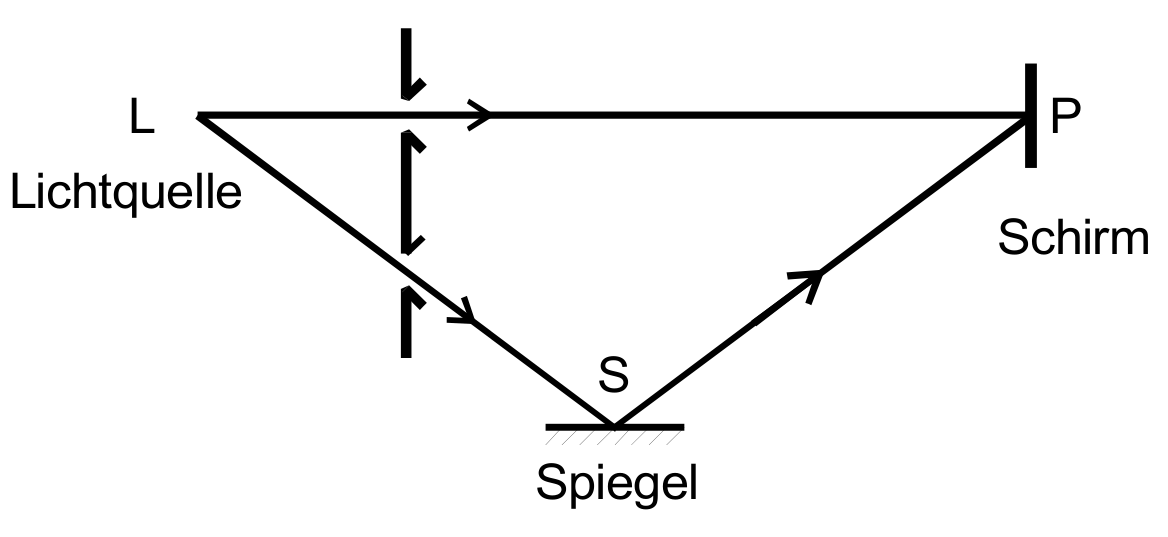
\includegraphics[height=4cm]{ressources/spaltung.png}
  \caption{Aufspaltung und Zusammenführung eines Lichtbündels\cite{Quelle0}.}
  \label{abb:1}
\end{figure}
Beträgt die Differenz der beiden Wege nun ungeradzahlige Vielfache der halben Wellenlänge,
\begin{equation}
  \Delta = (2n+1)\frac{\lambda}{2},
\end{equation}
so kommt es zu Auslöschungseffekten am Punkt P.
Wichtig ist dabei der Begriff der Kohärenzlänge $l$.
Bei der grundlegenden Lichterzeugung durch angeregte Atome dauert der Emissionsvorgang beschränkte Zeit.
Dementsprechend besitzt der Wellenzug eine endliche Länge, das Passieren dieses Wellenzuges entspricht einer bestimmten Zeit $\tau$.
%Bei mehreren Atomen (im Prinzip Lichtquellen) überlagern sich die Wellenzüge, welche sie emittieren.
%Da, wie bereits erwähnt, die Emission von Licht in endlichen Zeitintervallen $\tau$ stattfindet, hat der Wellenzug (bei mehreren Emittern die Wellengruppe) eine endliche Länge.
Wird diese Länge durch die Wegdifferenz überschritten, überlagern sich am Auftreffpunkt P zwei Wellenzüge von unterschiedlichen Emissionsakten, was bei hinreichend großem Wegunterschied zum Verschwinden des Interferenzeffektes führt.
Demnach wird die Kohärenzlänge festgelegt als das Produkt der bei P maximal beobachtbaren Intensitätsmaxima $N$ mit der Wellenlänge $\lambda$ des Lichtes,
\begin{equation}
  l = N\lambda.\\
\end{equation}
Laserlicht besitzt dabei, im Gegensatz zu einer herkömmlichen Lichtquelle, eine unendliche Kohärenzlänge, wenn bedacht wird, dass der Emissionsakt immer im Gleichtakt vollführt wird.\\
Zusätzlich kann die Breite der Lichtquelle zur Verhinderung der Interferenzerscheinungen führen, da das von verschiedenen Orten der Lichtquelle emittierte Licht im Allgemeinen durch die verschiedenen Richtungen zum Beobachtungspunkt eine Phasendifferenz besitzt.
Der Effekt kann durch die Verwendung eines großen Abstandes zur Lichtquelle oder durch die Verwendung einer kleinen Öffnung minimiert werden.
%%Dies wird als räumliche Inkohärenz aufgefasst.


%Die letzten zwei Sätze können wir auch rausnehmen.....Wahrscheinlich besser....LASS ES WEG!


\subsection{Wellenlängenmessung mittels Interferenz}

Die Quintessenz dieses Abschnittes lautet, dass sich die Wellenlänge einer Lichtquelle über eine Aufspaltung des Lichtes auf verschieden lange Wege, wobei einer um eine Strecke $\Delta l$ variiert wird, und anschließender Zusammenführung der Strahlen durch eine Zählung der entstehenden Interferenzmaxima bestimmen lässt.
Dies genügt der Gleichung
\begin{equation}
  \Delta l = N\frac{\lambda}{2}, \label{eqn:2}
\end{equation}
bei der $N$ die gezählten Interferenzmaxima beschreibt.\\

\subsection{Bestimmung eines Brechungsindex über Interferenz}

Befindet sich die Messapparatur in einem Medium, herrscht auf jeder Wegstrecke der Brechungsindex $n$.
Wird ein anderes Medium der Dicke $b$ einem Strahlengang in den Weg gesetzt, durchläuft das Licht auf diesem Ast eine zusätzliche effektive Weglänge von $b\Delta n$.
Dadurch lässt sich bei bekannter Wellenlänge die Änderung des Brechungsindex $\Delta n$,
\begin{equation}
  b\Delta n = N\frac{\lambda}{2}, \label{eqn:3}
\end{equation}
beschreiben.
Zur Berechnung des Brechungsindex unter Normalbedingungen wird die Formel
\begin{equation}
  n(p_0,T_0) = 1 +\Delta n(\Delta p) \frac{T}{T_0}\frac{p_0}{\Delta p}
\end{equation}
verwendet, bei der $p_0$ den Normaldruck und $T_0$ die Normaltemperatur beschreibt.
Wird diese Formel durch den Ausdruck (\ref{eqn:3}) ergänzt ergibt sich
\begin{equation}
  n(p_0,T_0) = 1 +\frac{N \lambda}{2b} \frac{T}{T_0}\frac{p_0}{\Delta p}, \label{eqn:soso}
\end{equation}
wobei $\lambda$ die Wellenlänge des Lasers und $b$ die Länge des Gasbehälters ist, welchen das Laserlicht passiert.





% 2x2 Plot
% \begin{figure*}
%     \centering
%     \begin{subfigure}[b]{0.475\textwidth}
%         \centering
%         \includegraphics[width=\textwidth]{Abbildungen/Schaltung1.pdf}
%         \caption[]%
%         {{\small Schaltung 1.}}
%         \label{fig:Schaltung1}
%     \end{subfigure}
%     \hfill
%     \begin{subfigure}[b]{0.475\textwidth}
%         \centering
%         \includegraphics[width=\textwidth]{Abbildungen/Schaltung2.pdf}
%         \caption[]%
%         {{\small Schaltung 2.}}
%         \label{fig:Schaltung2}
%     \end{subfigure}
%     \vskip\baselineskip
%     \begin{subfigure}[b]{0.475\textwidth}
%         \centering
%         \includegraphics[width=\textwidth]{Abbildungen/Schaltung4.pdf}    % Zahlen vertauscht ... -.-
%         \caption[]%
%         {{\small Schaltung 3.}}
%         \label{fig:Schaltung3}
%     \end{subfigure}
%     \quad
%     \begin{subfigure}[b]{0.475\textwidth}
%         \centering
%         \includegraphics[width=\textwidth]{Abbildungen/Schaltung3.pdf}
%         \caption[]%
%         {{\small Schaltung 4.}}
%         \label{fig:Schaltung4}
%     \end{subfigure}
%     \caption[]
%     {Ersatzschaltbilder der verschiedenen Teilaufgaben.}
%     \label{fig:Schaltungen}
% \end{figure*}
